\chapter{Sumator o dwóch wejściach}



\section{Dobranie oporników oraz budowa układu}

\begin{itemize}
    \item Zgodnie ze schematem sumatora (\ref{fig:schemat_sumatora}) należało zbudować sumator o 2 wejściach.
    \item Dobrano oraz zmierzono 3 oporniki:
        \begin{gather}
            \label{sumator:R1} R_1 = \textbf{2.96k}\boldsymbol{\Omega} \\
            \label{sumator:R2} R_2 = \textbf{2.97k}\boldsymbol{\Omega} \\
            \label{sumator:R3} R_3 = \textbf{2.98k}\boldsymbol{\Omega} 
        \end{gather}
    \item Używając schematu (\ref{fig:schemat_sumatora}) oraz oporników (\ref{sumator:R1}, \ref{sumator:R2}, \ref{sumator:R3}) zbudowano sumator. 
        \begin{figure}[H]
        \centering
        \begin{subfigure}[h]{0.4\textwidth}
            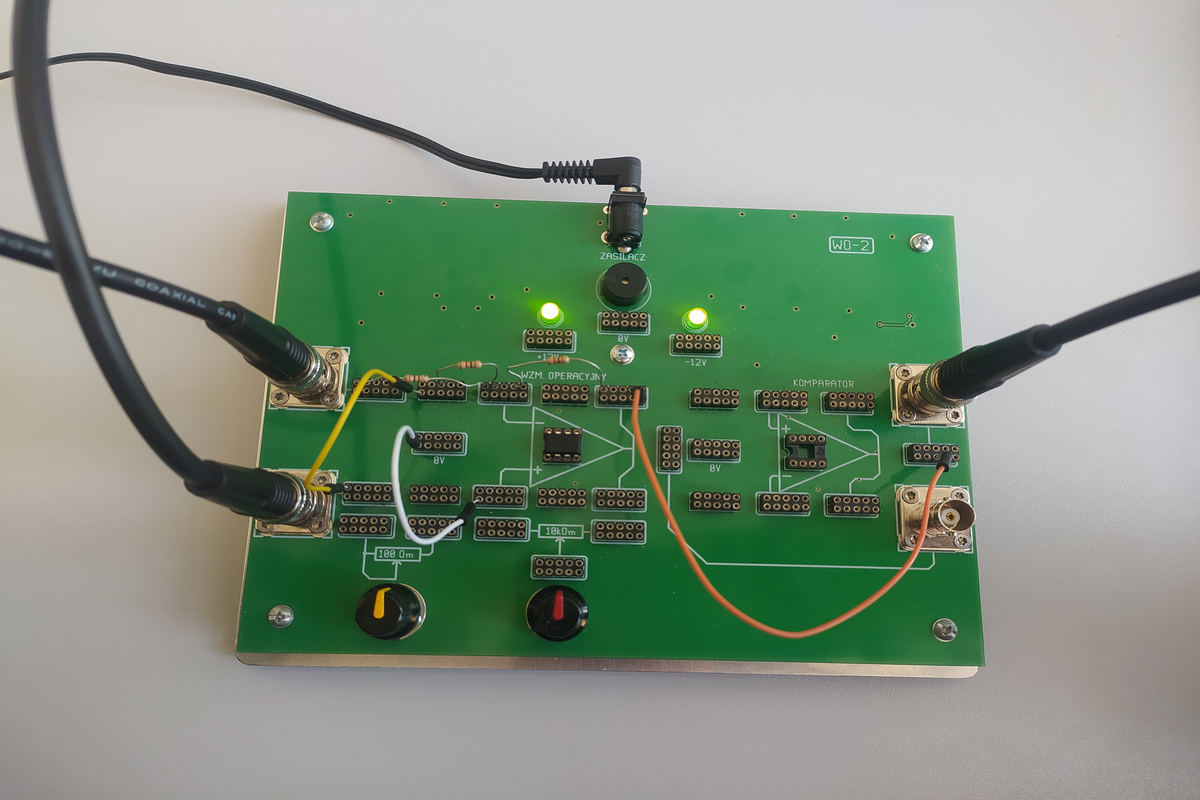
\includegraphics[width=\textwidth]{img/phone/1651502036847_scaled.png}
        \end{subfigure}
        \begin{subfigure}[h]{0.4\textwidth}
            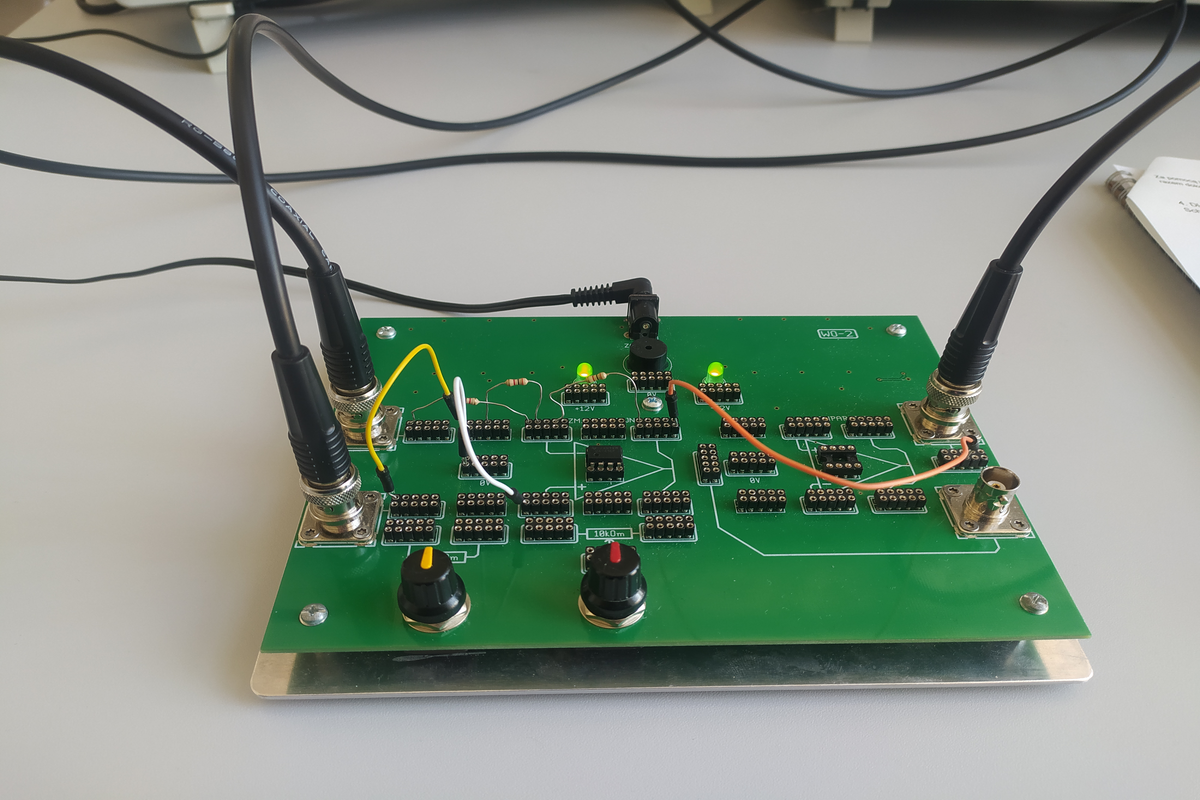
\includegraphics[width=\textwidth]{img/phone/1651502036824_scaled.png}
        \end{subfigure}
        \caption{Zmontowany układ}
        \label{sumator:zmontowany_uklad}
    \end{figure}
\end{itemize}

\section{Obserwacja dudnień}

\begin{itemize}
    \item Na płytkę przesłano dwa sygnały wejściowe o parametrach:
        \begin{itemize}
            \item Kanał 1:
                \begin{gather}
                    U_1 = \textbf{1V}, f_1 = \textbf{1kHz}
                \end{gather}
            \item Kanał 2:
                \begin{gather}
                    U_2 = \textbf{1V}, f_2 = \textbf{1.05kHz}
                \end{gather}
        \end{itemize}
    \item Sygnał wyjściowy poprowadzono do oscyloskopu co pozwoliło zaobserwować zjawisko dudnień.
        \begin{figure}[H]
            \centering
            \begin{subfigure}[h]{0.4\textwidth}
                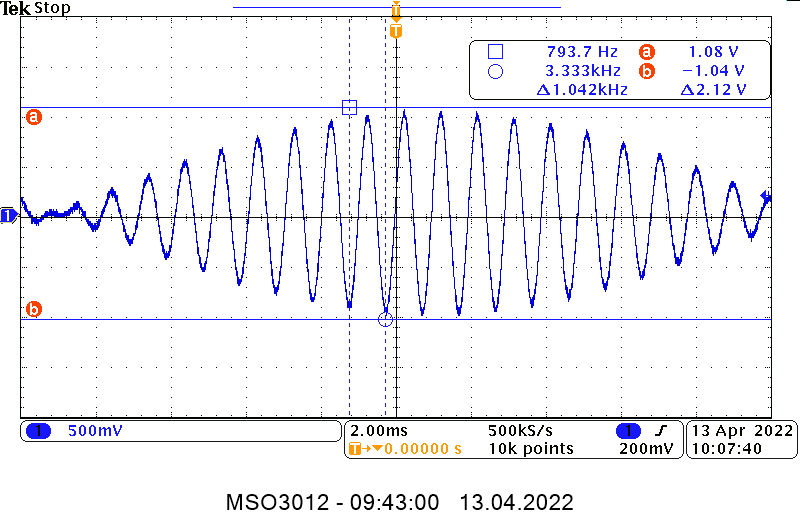
\includegraphics[width=\textwidth]{img/osciloscope/1_3_dudnienia2_cropped.png}
            \end{subfigure}
            \begin{subfigure}[h]{0.4\textwidth}
                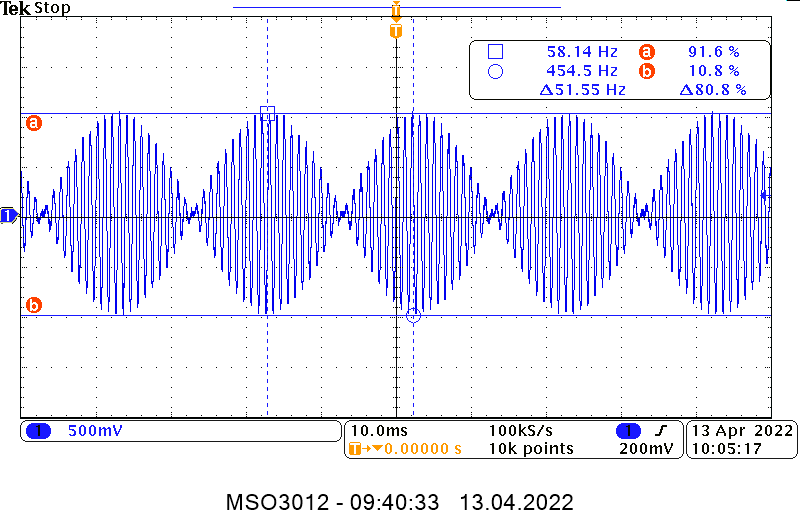
\includegraphics[width=\textwidth]{img/osciloscope/1_3_dudnienia_cropped.png}
            \end{subfigure}
            \caption{Zjawisko dudnień}
            \label{sumator:dudnienia}
        \end{figure}
    
    \item Teoretyczna wypadkowa częstotliwość przyjmuje wartość:
        \begin{equation}
            f_{wyp} = \frac{f_1 + f_2}{2} = \frac{2.05kHz}{2} = 1.025kHz = \textbf{1025Hz}
        \end{equation}
        \begin{center}
            Zmierzona wartość wyniosła 1.042kHz = \textbf{1042Hz}
        \end{center}
        \begin{center}
            Różnica $\Delta_f$ = $f_{wyp}$ - $f_{zmierzona}$ = \textbf{17Hz}
        \end{center}
        \begin{figure}[H]
            \centering
            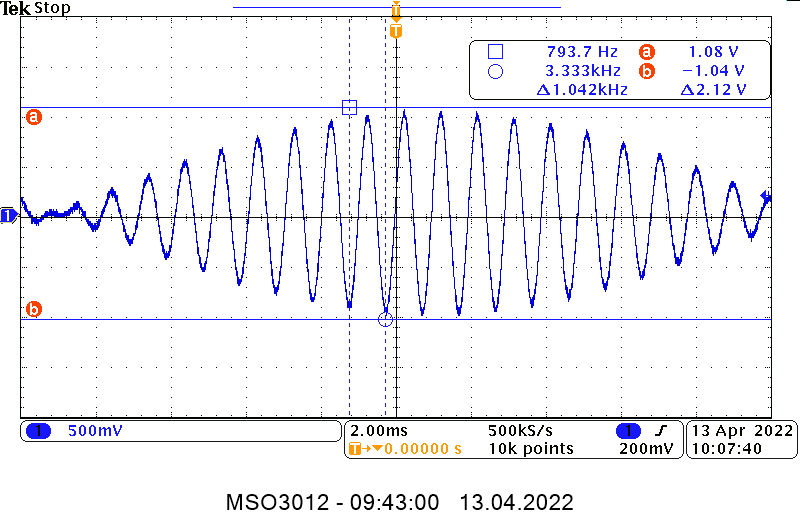
\includegraphics[scale=0.33]{img/osciloscope/1_3_dudnienia2_cropped.png}
            \caption{Wypadkowa częstotliwość zmierzona za pomocą kursorów}
            \label{fig:wypadkowa}
        \end{figure}
        
    \item Częstotliwość dudnienia zmierzono za pomocą kursorów. Przewidywana wartość wynosiła:
        \begin{equation}
            f_{dud} = |f_1 - f_2| = 0.05kHz = \textbf{50Hz}
        \end{equation}
        \begin{center}
            Zmierzona wartość wyniosła \textbf{51.55Hz} \\
            Różnica $\Delta_{dud}$ = $f_{wyp}$ - $f_{zmierzona}$ = \textbf{1.55Hz}
        \end{center}
        \begin{figure}[h]
            \centering
            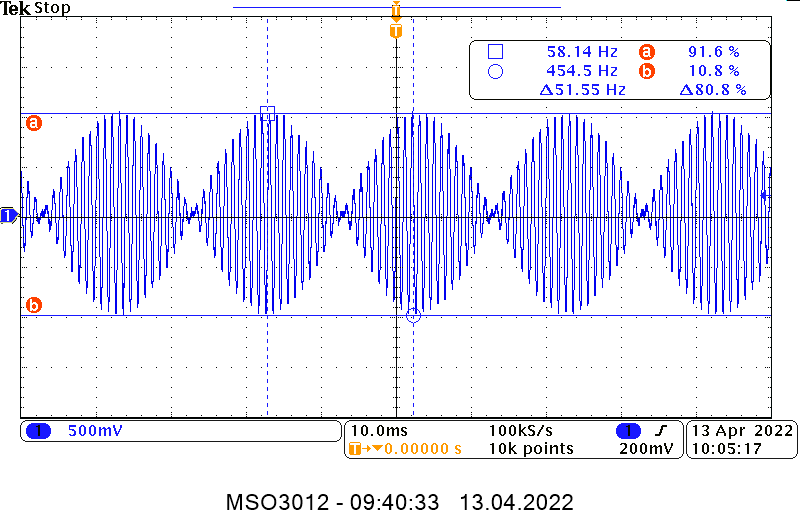
\includegraphics[scale=0.33]{img/osciloscope/1_3_dudnienia_cropped.png}
            \caption{Pomiar częstotliwości dudnień za pomocą kursorów}
            \label{fig:cz_dudnienia}
        \end{figure}
\end{itemize}